% M-DaQ Poster for SIGIR 2026
% Generated for Overleaf compilation
% A0 Portrait, 2-column layout
% 
% COMPILER: XeLaTeX (required for fontspec)
% In Overleaf: Menu → Compiler → XeLaTeX

\documentclass[final]{beamer}

% ====================
% Packages
% ====================
\usepackage[T1]{fontenc}
\usepackage{lmodern}
\usepackage[size=custom,width=84.1,height=118.9,scale=1.0]{beamerposter}
\usetheme{gemini}
\usecolortheme{cam}
\usepackage{graphicx}
\usepackage{booktabs}
\usepackage[numbers]{natbib}
\usepackage{tikz}
\usepackage{pgfplots}
\pgfplotsset{compat=1.14}
\usepackage{anyfontsize}
\usepackage{fontspec}

% ====================
% Custom Colors
% ====================
\definecolor{mdaqblue}{RGB}{27, 58, 92}
\definecolor{mdaqorange}{RGB}{232, 121, 43}
\definecolor{lightbg}{RGB}{240, 244, 248}

\setbeamercolor{headline}{bg=white, fg=mdaqblue}
\setbeamercolor{block title}{bg=mdaqblue, fg=white}
\setbeamercolor{block body}{bg=white, fg=black}
\setbeamercolor{block title example}{bg=mdaqorange, fg=white}

\addtobeamertemplate{block begin}{
  \setlength{\textpaddingtop}{0.3em}%
  \setlength{\textpaddingbottom}{0.3em}%
}{}

% ====================
% Layout: 2 columns
% (N+1)*sepwidth + N*colwidth = paperwidth
% 3*sepwidth + 2*colwidth = 84.1cm
% sepwidth = 0.03 * 84.1 = 2.523cm
% colwidth = (84.1 - 3*2.523) / 2 = 38.26cm
\newlength{\sepwidth}
\newlength{\colwidth}
\setlength{\sepwidth}{0.03\paperwidth}
\setlength{\colwidth}{0.47\paperwidth}

\newcommand{\separatorcolumn}{\begin{column}{\sepwidth}\end{column}}

% ====================
% Title & Authors
% ====================
\title{\huge M-DaQ: Retrieving Samples with Multilingual Diversity and Quality for Instruction Fine-Tuning Datasets}

\author{
  Chunguang Zhao\textsuperscript{1} \and
  Yilun Liu\textsuperscript{1} \and
  Pufan Zeng\textsuperscript{2} \and
  Yuanchang Luo\textsuperscript{1} \and
  Shimin Tao\textsuperscript{1} \and
  Minggui He\textsuperscript{1} \and
  Weibin Meng\textsuperscript{1} \and
  Song Xu\textsuperscript{2} \and
  Chen Liu\textsuperscript{1} \and
  Hongxia Ma\textsuperscript{1} \and
  Li Zhang\textsuperscript{1} \and
  Boxing Chen\textsuperscript{1} \and
  Daimeng Wei\textsuperscript{1}
}

\institute[shortinst]{
  \textsuperscript{1} Huawei Technologies Ltd. \samelineand
  \textsuperscript{2} University of Science and Technology of China
}

% ====================
% Footer
% ====================
\footercontent{
  \href{https://doi.org/10.1145/3805712.3809946}{DOI: 10.1145/3805712.3809946} \hfill
  SIGIR 2026 $\cdot$ Melbourne, Australia $\cdot$ July 20--24, 2026 \hfill
  \href{https://github.com/zhaocorey/M-DaQ}{github.com/zhaocorey/M-DaQ}
}

% ====================
% Logos (Huawei left, SIGIR + USTC stacked right)
% ====================
\logoleft{
\includegraphics[height=3.5cm]{logos/huawei_logo.png}}
\logoright{
  \begin{minipage}{8cm}
    \centering
    
\includegraphics[height=3cm]{logos/sigir_logo.png}\\[0.5em]
    
\includegraphics[height=2cm]{logos/ustc_logo.png}
  \end{minipage}
}

% ====================
% Body
% ====================
\begin{document}

\begin{frame}[t]
\begin{columns}[t]
\separatorcolumn

% ============================================================
% COLUMN 1 (LEFT)
% ============================================================
\begin{column}{\colwidth}

  % ---- MOTIVATION ----
  \begin{block}{\Large 1\quad Motivation}
    \textbf{The Problem:} Multilingual instruction fine-tuning (IFT) data is scarce, heavily skewed toward English, and lacks systematic curation.

    \vspace{0.5em}
    \begin{itemize}
      \item Llama-3 IFT dataset contains only \textbf{3.01\%} multilingual samples
      \item No language-agnostic quality scoring method exists for multilingual data
      \item Data diversity has been studied only in English settings
      \item The Superficial Alignment Hypothesis (SAH) remains unverified in multilingual contexts
    \end{itemize}

    \vspace{0.8em}
    \textbf{Three Challenges Addressed:}

    \vspace{0.3em}
    \begin{center}
    \begin{tabular}{p{0.12\textwidth} p{0.38\textwidth} p{0.4\textwidth}}
      \toprule
      \textbf{Challenge} & \textbf{Problem} & \textbf{M-DaQ Solution} \\
      \midrule
      C1 & No extensible quality scoring for multilingual IFT & Quality Scoring Model (QSM) with triplet loss \\
      C2 & Diversity selection limited to English & Diversity-Aware Selection (DAS) inspired by MMR \\
      C3 & SAH unverified in multilingual settings & Systematic 1K$\to$52K scale study across 8 languages \\
      \bottomrule
    \end{tabular}
    \end{center}
  \end{block}

  % ---- METHOD ----
  \begin{block}{\Large 2\quad Method: M-DaQ Framework}

    \textbf{\textcolor{mdaqorange}{Stage 1: Quality Scoring Model (QSM)}}
    \begin{itemize}
      \item Fine-tuned on \textbf{$\sim$2.3K expert-revised samples $\times$ 18 languages} (from MIDB)
      \item \textbf{Triplet loss}: instruction $\to$ positive (expert-revised) vs.\ negative (original/MT)
      \item Learns language-agnostic quality signal from embedding space
    \end{itemize}

    \vspace{0.8em}
    \textbf{\textcolor{mdaqorange}{Stage 2: Diversity-Aware Selection (DAS)}}
    \begin{itemize}
      \item \textbf{MMR-inspired}: Quality $\approx$ Relevance, Diversity $\approx$ Novelty
      \item Two-stage pipeline reduces $\mathcal{O}(n^2) \to \mathcal{O}(n \log n)$:
      \begin{itemize}
        \item Stage A: Select top-$n$ by QSM score (quality subset)
        \item Stage B: Greedily augment from uncovered clusters (diversity subset)
      \end{itemize}
      \item Ratio $n_{\text{quality}} : n_{\text{diversity}} = \mathbf{6:1}$ (empirically tuned)
    \end{itemize}
  \end{block}

  % ---- PIPELINE FIGURE ----
  \begin{block}{\Large M-DaQ Pipeline}
    \begin{center}
      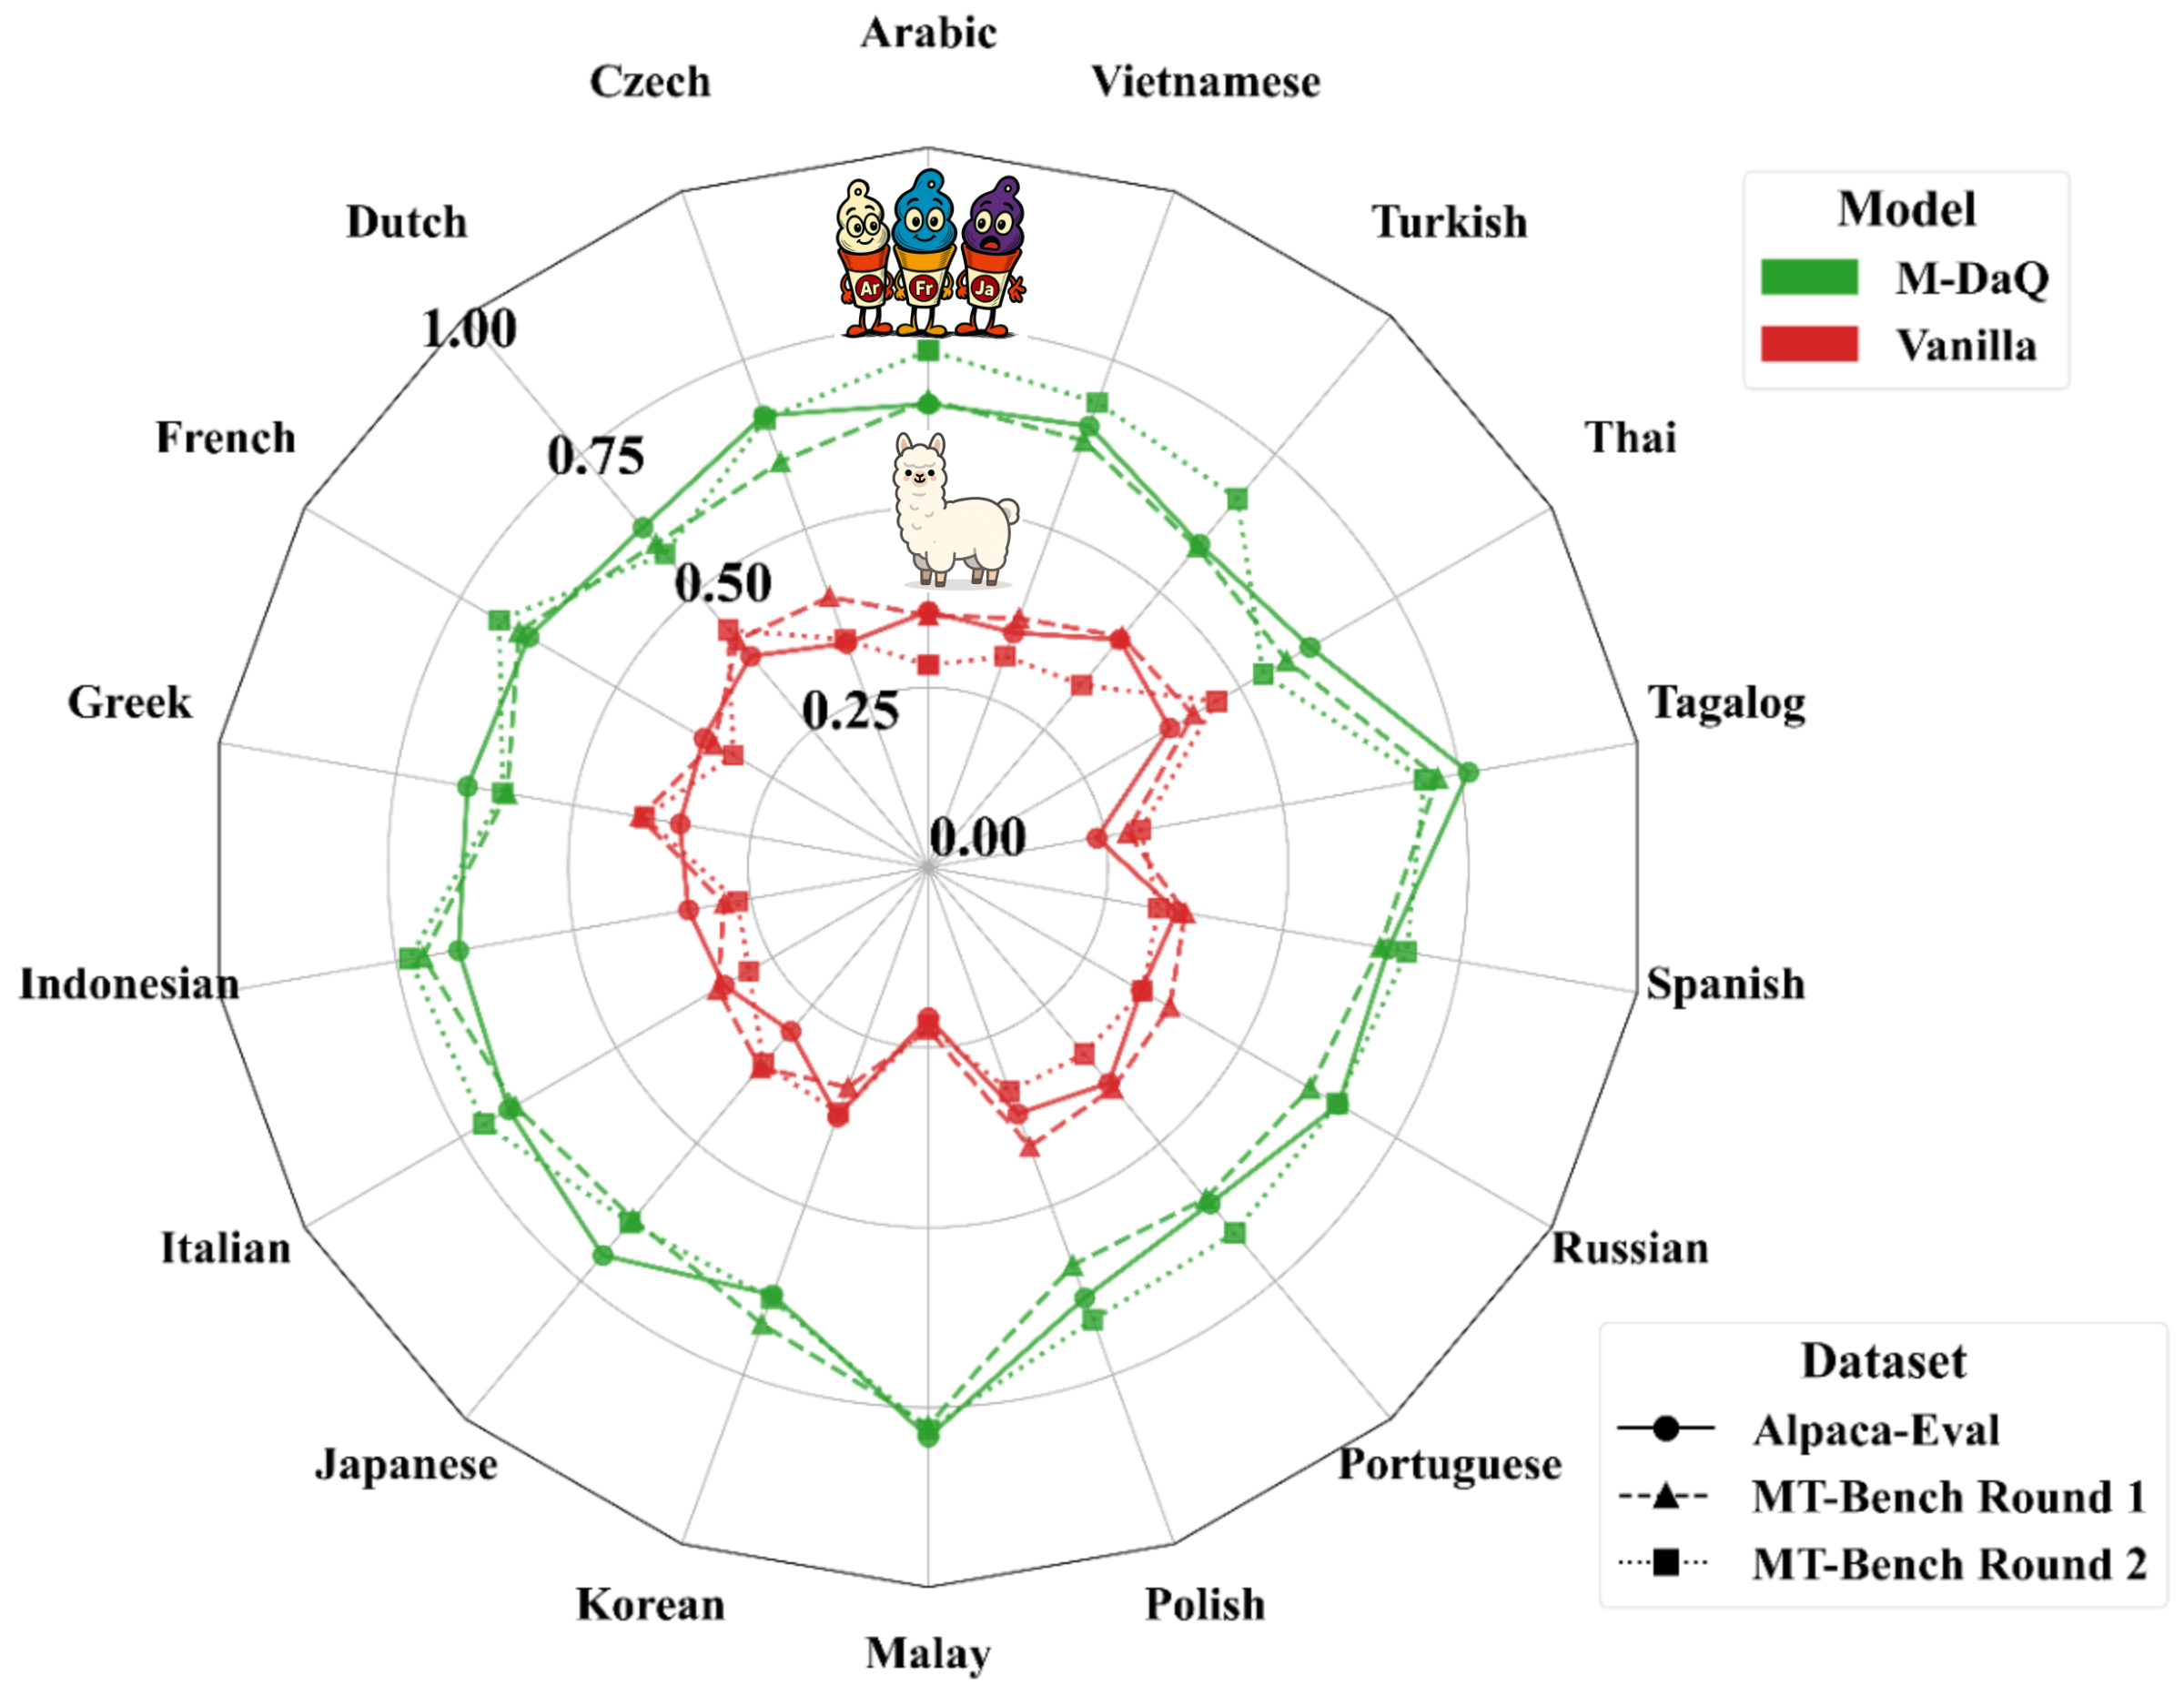
\includegraphics[width=0.92\textwidth]{figures/pipeline.png}
      \vspace{0.3em}
      {\small \textit{Figure: M-DaQ two-stage pipeline (QSM + DAS). Stage 1 scores quality via triplet loss; Stage 2 selects diverse samples via greedy cluster augmentation.}}
    \end{center}
  \end{block}

\end{column}

\separatorcolumn

% ============================================================
% COLUMN 2 (RIGHT)
% ============================================================
\begin{column}{\colwidth}

  % ---- KEY RESULTS ----
  \begin{block}{\Large 3\quad Key Results}

    \begin{center}
    \colorbox{lightbg}{
      \begin{minipage}{0.95\textwidth}
        \centering
        \textbf{LLM-as-Judge: Avg Win Rate (M-DaQ vs.\ Vanilla)}\\[0.5em]
        \Large
        \textbf{Alpaca-Eval: 60.2\%} \quad $\cdot$ \quad
        \textbf{MT-Bench R1: 62.6\%} \quad $\cdot$ \quad
        \textbf{MT-Bench R2: 62.9\%}
      \end{minipage}
    }
    \end{center}

    \vspace{0.8em}
    \begin{center}
      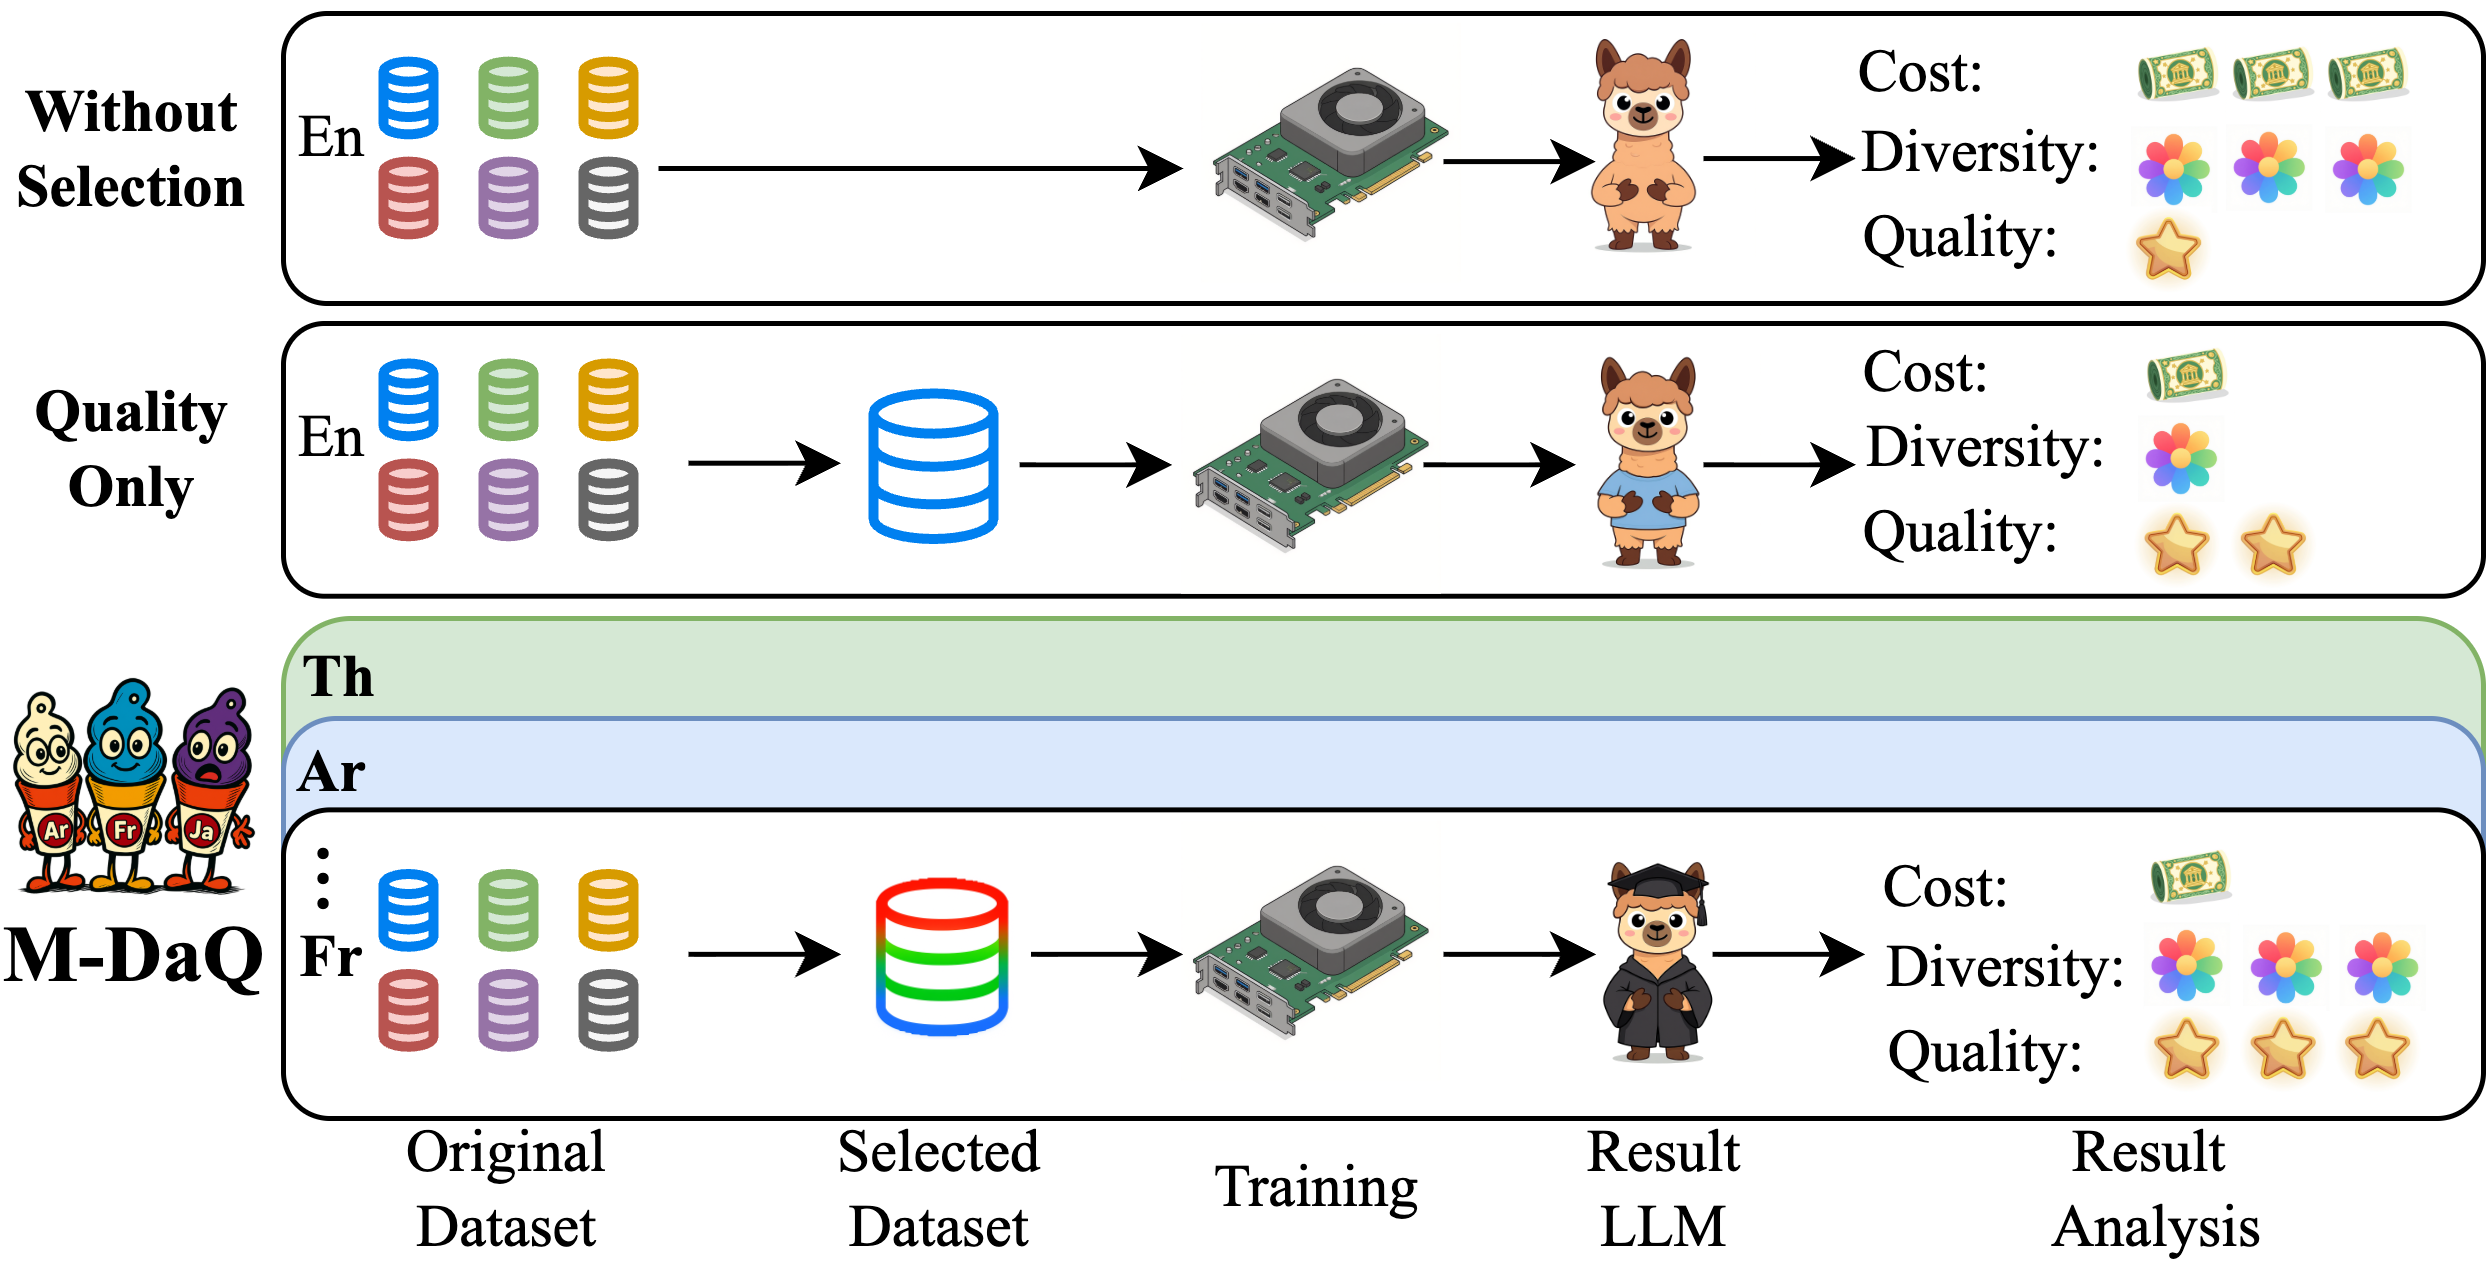
\includegraphics[width=0.92\textwidth]{figures/win_rates_18langs.png}
      \vspace{0.2em}
      {\small \textit{Figure: Cross-lingual win rates across 18 languages (Alpaca-Eval + MT-Bench). Gains are more pronounced in low-resource languages.}}
    \end{center}

    \vspace{0.5em}
    \textbf{Key Observations:}
    \begin{itemize}
      \item Consistent improvement across all 18 languages
      \item Gains \textbf{more pronounced} in low-resource languages (Tagalog, Malay)
      \item M-DaQ effectively mitigates linguistic imbalance and data scarcity
    \end{itemize}
  \end{block}

  % ---- HUMAN EVALUATION ----
  \begin{block}{\Large 4\quad Human Evaluation}
    \textbf{Setup:} 6 Languages $\cdot$ 900 Samples $\cdot$ 58 Person-Hours

    \vspace{0.5em}
    \begin{center}
    \begin{tabular}{l c c c}
      \toprule
      \textbf{Language} & \textbf{Alpaca-Eval} & \textbf{MT-Bench R1} & \textbf{MT-Bench R2} \\
      \midrule
      Japanese      & 86\% & 84\% & 80\% \\
      Korean        & 94\% & 94\% & 94\% \\
      Russian       & 70\% & 86\% & 84\% \\
      Portuguese    & 80\% & 78\% & 84\% \\
      Greek         & 58\% & 76\% & 82\% \\
      French        & 80\% & 92\% & 88\% \\
      \midrule
      \textbf{Average} & \textbf{78.0\%} & \textbf{85.0\%} & \textbf{85.3\%} \\
      \bottomrule
    \end{tabular}
    \end{center}
  \end{block}

  % ---- SAH VALIDATION ----
  \begin{block}{\Large 5\quad SAH in Multilingual Settings}
    \textit{First systematic investigation of the Superficial Alignment Hypothesis across languages.}

    \vspace{0.5em}
    \begin{center}
      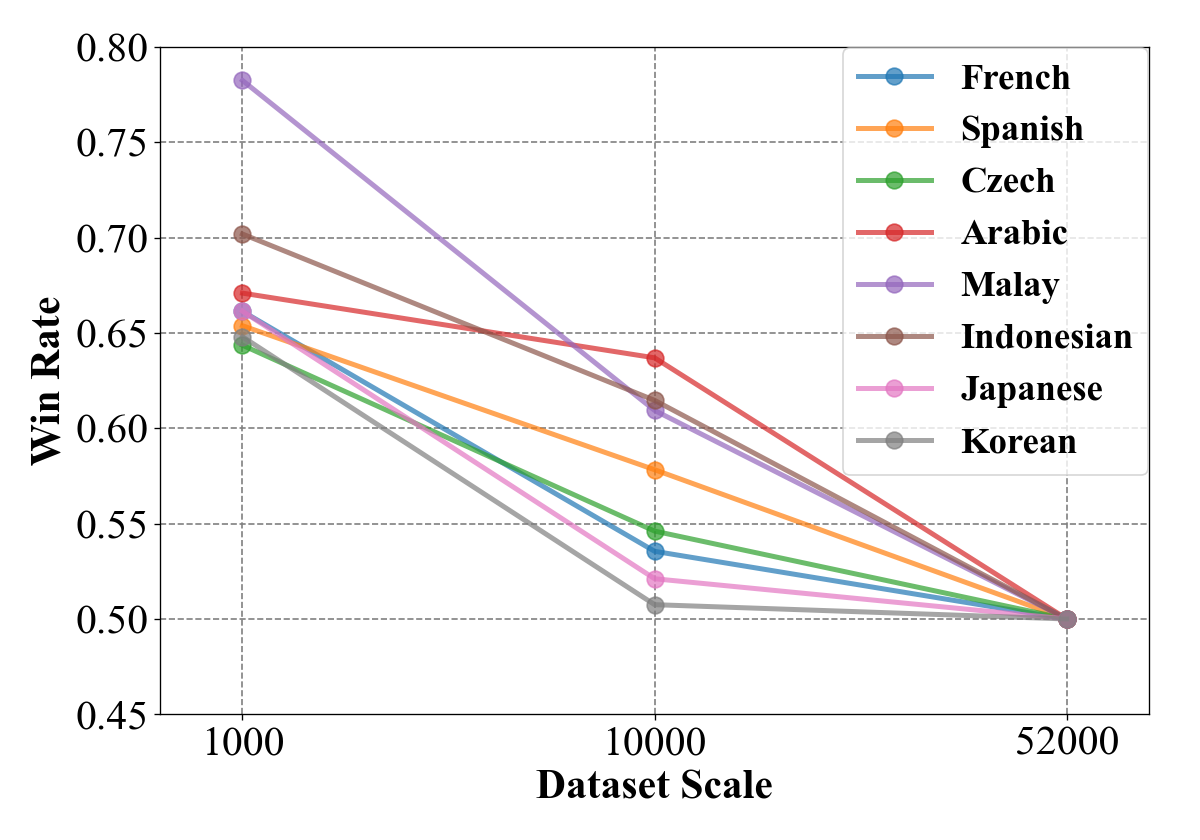
\includegraphics[width=0.85\textwidth]{figures/sah_scale.png}
      \vspace{0.2em}
      {\small \textit{Figure: Win rate vs.\ IFT dataset scale (1K--52K), 8 languages.}}
    \end{center}

    \vspace{0.5em}
    \textbf{Key Findings:}
    \begin{itemize}
      \item \textbf{Diminishing returns}: 1K curated $>$ 52K unfiltered --- SAH holds multilingually
      \begin{itemize}
        \item 10K $\to$ $-10.1\%$ avg win rate vs.\ 1K baseline
        \item 52K $\to$ $-6.2\%$ avg win rate vs.\ 1K baseline
      \end{itemize}
      \item \textbf{Language-dependent sensitivity}: Arabic shows flatter curve than French (lower pretraining readiness)
      \item \textbf{Practical implication}: A few thousand high-quality samples suffice for effective multilingual alignment
    \end{itemize}
  \end{block}

  % ---- CONCLUSION ----
  \begin{block}{\Large 6\quad Conclusion}
    \begin{itemize}
      \item \textbf{M-DaQ = QSM + DAS}: compact, high-fidelity multilingual IFT subsets
      \item \textbf{60\%+ avg win rate} across 18 languages on Alpaca-Eval \& MT-Bench
      \item Human evaluation confirms gains in \textbf{cultural relevance}, contextual appropriateness, instruction-following
      \item First empirical validation of \textbf{SAH in multilingual settings}
      \item Code released: \href{https://github.com/zhaocorey/M-DaQ}{github.com/zhaocorey/M-DaQ}
    \end{itemize}
  \end{block}

  % ---- CONTACT ----
  \begin{block}{\Large Contact \& Resources}
    \begin{columns}[t]
      \begin{column}{0.5\textwidth}
        \textbf{Paper:}\\
        DOI: \href{https://doi.org/10.1145/3805712.3809946}{10.1145/3805712.3809946}\\
        arXiv: 2509.15549
      \end{column}
      \begin{column}{0.5\textwidth}
        \textbf{Contact:}\\
        zhaochunguang6@huawei.com\\
        +86-15501192353
      \end{column}
    \end{columns}
  \end{block}

\end{column}

\separatorcolumn
\end{columns}
\end{frame}

\end{document}
